% ============================================================
% Section 4: Experiments and Results
% ============================================================

\section{Experiments and Results}
\label{sec:experiments}

\subsection{Experimental Setup}
\label{subsec:setup}

All experiments are conducted on a single NVIDIA RTX~5060\,Ti (16\,GB VRAM) under
Windows~11, using PyTorch 2.10.0 with CUDA 13.0 and Optuna~3.x. The full nested
cross-validation pipeline (including 2\,500 HPO trials and 10 final models) required
approximately 59 hours of wall-clock time. The scalar experiment
(Section~\ref{subsec:scalar}) required an additional 4.6 hours.

Images are loaded into GPU memory at the start of each outer fold to eliminate
CPU-to-GPU transfer overhead during inner-fold HPO trials (per-fold VRAM cache).
This optimization reduced per-trial training time from approximately 12 to 3.5 minutes.

\subsection{Nested Cross-Validation Results}
\label{subsec:ncv_results}

Table~\ref{tab:nested_cv} reports the per-fold test metrics obtained from the 10
outer folds of the nested cross-validation. Each metric is computed on the held-out
test fold using the model trained with the Pareto-selected hyperparameter
configuration.

\begin{table*}[!t]
  \centering
  \caption{Per-fold test results from 10-fold nested cross-validation.
           $\overline{w}_{\text{mask}}$: Pareto-selected mask loss weight.}
  \label{tab:nested_cv}
  \begin{tabular}{ccccccc}
    \toprule
    Fold & PR-AUC & Dice & ROC-AUC & BACC & $\overline{w}_{\text{mask}}$ \\
    \midrule
    F1  & 0.9939 & 0.861 & 0.9848 & 0.9491 & 2.46 \\
    F2  & 0.9769 & 0.871 & 0.9615 & 0.9319 & 2.70 \\
    F3  & 0.9993 & 0.909 & 0.9981 & 0.9470 & 2.47 \\
    F4  & 0.9915 & 0.858 & 0.9773 & 0.8986 & 2.43 \\
    F5  & 0.9948 & 0.827 & 0.9869 & 0.9318 & 1.41 \\
    F6  & 0.9936 & 0.874 & 0.9830 & 0.9319 & 2.89 \\
    F7  & 0.9940 & 0.861 & 0.9834 & 0.9479 & 2.67 \\
    F8  & 0.9967 & 0.887 & 0.9911 & 0.9557 & 2.29 \\
    F9  & 0.9896 & 0.807 & 0.9722 & 0.9023 & 1.95 \\
    F10 & 0.9909 & 0.800 & 0.9765 & 0.9294 & 2.65 \\
    \midrule
    \textbf{Mean} & \textbf{0.9921} & \textbf{0.856} & \textbf{0.9815} & \textbf{0.9326} & \textbf{2.39} \\
    \textbf{Std}  & \textbf{0.0058} & \textbf{0.030} & \textbf{0.0110} & \textbf{0.0192} & \textbf{0.43} \\
    \bottomrule
  \end{tabular}
\end{table*}

PR-AUC is consistently high across all folds ($0.977$--$0.999$, mean
$0.9921 \pm 0.0058$), confirming reliable document-level detection generalization.
Dice scores show slightly more fold-to-fold variability ($0.800$--$0.909$, mean
$0.856 \pm 0.030$), reflecting the inherent difficulty of pixel-level localization
under diverse forgery patterns. No fold exhibits a performance collapse, confirming
that the model does not over-fit to any particular subset of the training
distribution.

The Pareto-selected $\lambda_{\text{mask}}$ values cluster consistently between
2.3 and 2.7 (eight of ten folds), with folds F5 and~F9 selecting lower weights
(1.41 and~1.95), which coincide with the two lowest Dice scores in the table.
This observation suggests that $\lambda_{\text{mask}}$ plays a decisive role in
localization quality and motivates including it in the HPO search space rather
than fixing it a priori.

Figure~\ref{fig:nested_cv} visualizes the per-fold PR-AUC and Dice values with
their cross-fold means.

\begin{figure*}[!t]
  \centering
  
\includegraphics[width=\textwidth]{fig2_nested_cv}
  \caption{Per-fold test metrics from 10-fold nested cross-validation. Blue bars:
    PR-AUC; orange bars: Dice. Dashed lines indicate cross-fold means
    (PR-AUC $= 0.9921 \pm 0.0060$; Dice $= 0.8555 \pm 0.0345$). The $y$-axis
    is truncated at $0.75$ to emphasize fold-to-fold variation.}
  \label{fig:nested_cv}
\end{figure*}

\subsection{Ablation Study}
\label{subsec:ablation}

\subsubsection{Variants}
To isolate the contribution of each design decision, we evaluate four model
variants on the blind test set using 30 independent random seeds per variant:

\begin{itemize}
  \item \textbf{Multitask} (proposed): joint detection + localization with
        Pareto-optimized $\lambda_{\text{mask}}$.
  \item \textbf{cls\_only}: classification head only; no segmentation head or
        segmentation loss.
  \item \textbf{seg\_only}: segmentation head only; classification is performed
        by thresholding the mean mask probability.
  \item \textbf{unweighted\_losses}: full multitask architecture with equal
        task weights ($\lambda_{\text{cls}} = \lambda_{\text{mask}} = 0.5$),
        bypassing HPO entirely.
\end{itemize}

\subsubsection{Results}
\label{sec:blindtest}

Table~\ref{tab:ablation} reports mean and standard deviation over 30 seeds for
PR-AUC and Dice, along with Wilcoxon signed-rank tests with Holm--Bonferroni
correction comparing each variant to the Multitask baseline.
Effect sizes are reported as Cohen's $d$~\cite{cohen1988statistical}.

\begin{table*}[htbp]
  \centering
  \caption{Ablation study results (blind test, 30 seeds).
           $p$: Wilcoxon signed-rank with Holm correction; $d$: Cohen's $d$.
           Significance: *** $p < 0.001$; ns $p \geq 0.05$.}
  \label{tab:ablation}
  \begin{tabular}{lcccccc}
    \toprule
    & \multicolumn{2}{c}{PR-AUC} & \multicolumn{4}{c}{Dice} \\
    \cmidrule(r){2-3} \cmidrule(l){4-7}
    Variant & Mean $\pm$ Std & vs.\ Multitask & Mean $\pm$ Std & vs.\ Multitask & $p_{\text{holm}}$ & $d$ \\
    \midrule
    \textbf{Multitask} (ours) & $\mathbf{0.9967 \pm 0.0021}$ & — & $\mathbf{0.875 \pm 0.018}$ & — & — & — \\
    cls\_only          & $0.9503 \pm 0.0744$ & *** & $0.002 \pm 0.008$ & *** & $1.3 \times 10^{-8}$ & large \\
    seg\_only          & $0.7277 \pm 0.0528$ & *** & $0.867 \pm 0.023$ & ns  & $0.288$              & small \\
    unweighted\_losses & $0.9958 \pm 0.0016$ & ns  & $0.857 \pm 0.016$ & *** & $1.3 \times 10^{-4}$ & 1.01 \\
    \bottomrule
  \end{tabular}
\end{table*}

The results confirm three design choices. First, the joint multitask objective is
essential: \textbf{cls\_only} produces near-zero Dice ($0.002 \pm 0.008$),
confirming that the segmentation head cannot be removed without catastrophic
localization failure. Second, a dedicated classification head is necessary:
\textbf{seg\_only} achieves competitive Dice ($0.867$) but its PR-AUC drops to
$0.728 \pm 0.053$, demonstrating that the segmentation logit alone is an
insufficient detection signal. Third, the Pareto-optimized loss weights provide a
measurable benefit over equal weights: \textbf{unweighted\_losses} matches
Multitask on PR-AUC ($p = 0.083$, not significant) but shows significantly lower
Dice ($p = 1.3 \times 10^{-4}$, $d = 1.01$, large effect), validating the
contribution of the HPO weighting scheme specifically for localization quality.

Figure~\ref{fig:ablation} shows the distribution of scores across 30 seeds as
violin plots.

\begin{figure*}[!t]
  \centering
  
\includegraphics[width=\textwidth]{fig3_ablation}
  \caption{Ablation study: violin plots of PR-AUC (left) and Dice (right) for
    four variants over 30 seeds on the blind test set. Significance symbols above
    each violin denote Wilcoxon + Holm vs.\ Multitask (*** $p < 0.001$;
    ns $p \geq 0.05$).}
  \label{fig:ablation}
\end{figure*}

\subsection{Pareto HPO vs.\ Scalar Baselines}
\label{subsec:scalar}

To further contextualize the multi-objective HPO, we compare Pareto-based
selection against two scalar alternatives that select a configuration from the
same 50 MOTPE trials by maximizing a single inner-validation metric:
\textbf{by\_prauc} (maximize PR-AUC) and \textbf{by\_dice} (maximize Dice).

\begin{table*}[!t]
  \centering
  \caption{Comparison of HPO selection criteria on nested CV (10 folds).
           Wilcoxon + Holm vs.\ Pareto baseline; ns $p \geq 0.05$.}
  \label{tab:scalar}
  \begin{tabular}{lcccc}
    \toprule
    Method & PR-AUC & Dice & $p$ (PR-AUC) & $p$ (Dice) \\
    \midrule
    \textbf{Pareto (ours)} & $0.9921 \pm 0.0060$ & $0.8555 \pm 0.0345$ & — & — \\
    Scalar by\_prauc & $0.9958 \pm 0.0015$ & $0.8574 \pm 0.0166$ & ns & ns \\
    Scalar by\_dice  & $0.9936 \pm 0.0033$ & $0.8630 \pm 0.0147$ & ns & ns \\
    \bottomrule
  \end{tabular}
\end{table*}

No statistically significant differences are found between Pareto and either scalar
criterion (all $p \geq 0.05$, Wilcoxon + Holm, $n = 10$). The three methods
achieve closely matched absolute performance, with differences below $0.004$ on
PR-AUC and $0.008$ on Dice. Pareto selection shows higher variance in Dice
(std~$0.035$ vs.\ $0.015$--$0.017$ for scalar methods), which can be attributed to
sensitivity to inner-fold composition in folds where the Pareto-optimal
$\lambda_{\text{mask}}$ departs from the cluster mode (F5, F9).

The key advantage of Pareto HPO is therefore methodological rather than numerical:
it (i)~selects configurations without privileging either objective a priori,
consistently with the DeepID evaluation protocol; (ii)~makes the detection-localization
trade-off explicit through the Pareto front (Fig.~\ref{fig:pareto}), enabling
practitioners to choose alternative operating points; and (iii)~requires no
post-hoc justification for the selection criterion.

Figure~\ref{fig:scalar} shows the distribution of per-fold scores for all three
selection strategies.

\begin{figure*}[!t]
  \centering
  
\includegraphics[width=\textwidth]{fig5_scalar_vs_pareto}
  \caption{Pareto HPO vs.\ scalar selection on nested CV (10 folds). Box plots of
    PR-AUC (left) and Dice (right); jittered dots show individual fold results.
    Significance vs.\ Pareto: ns $p \geq 0.05$ (Wilcoxon + Holm, $n = 10$).}
  \label{fig:scalar}
\end{figure*}

\subsection{Comparison with DeepID 2025 Challenge Participants}
\label{subsec:challenge}

Table~\ref{tab:challenge} compares DocVerify against the top participants of the
DeepID 2025 Challenge on Track~1 (detection F1 at threshold 0.5) and Track~2
(per-image pixel-level F1). Challenge metrics are computed using
our challenge evaluation script over our internal holdout test split
(15\% of FantasyID) and 30 random seeds.

\begin{table*}[htbp]
  \centering
  \caption{Comparison with DeepID 2025 Challenge participants and related work.
           $\dagger$: evaluated on the official challenge test set;
           $\ddagger$: reported on FantasyID validation set (Dice coefficient);
           DocVerify evaluated on an internal 15\% holdout (see text).
           ``—'' indicates metric not reported or track not entered.}
  \label{tab:challenge}
  \begin{tabular}{lcccc}
    \toprule
    System & F1 det (thr=0.5) & F1 loc (per-image) & Training Data \\
    \midrule
    Sunlight~\cite{remtkd2025} (1st)$^\dagger$       & 0.991 & 0.784 & 60K+ external images \\
    Incode (2nd)$^\dagger$                            & 0.868 & —     & 100K proprietary images \\
    AG / EdgeDoc~\cite{edgedoc2025} (3rd)$^\dagger$  & 0.958 & 0.686 & FantasyID only \\
    UAM-Biometrics (4th)$^\dagger$                    & 0.712 & 0.620 & FantasyID only \\
    TruFor~\cite{trufor2023} baseline$^\dagger$       & 0.807 & 0.590 & 876K pre-training images \\
    TwoHead-SwinFPN~\cite{twoheadswin2026}$^\ddagger$ & —     & 0.572 & FantasyID only \\
    \midrule
    \textbf{DocVerify (ours)}       & $\mathbf{0.969 \pm 0.014}$ & $\mathbf{0.807 \pm 0.096}$ & FantasyID only \\
    \bottomrule
  \end{tabular}
\end{table*}

\textbf{Track 1 (detection).} DocVerify achieves $\text{F1}@0.5 = 0.969 \pm 0.014$,
surpassing all systems that trained exclusively on FantasyID, including AG/EdgeDoc
($+1.1$ pp) and UAM-Biometrics ($+25.7$~pp), and outperforming Incode despite
the latter using 100K proprietary images. The gap to Sunlight ($-2.2$~pp) is
attributable to Sunlight's use of over 60K additional external training images and
multi-stage pre-training.

\textbf{Track 2 (localization).} DocVerify achieves $\text{F1}_{\text{loc}} =
0.807 \pm 0.096$, which exceeds all four challenge finishers including the overall
winner Sunlight ($0.784$). This is the strongest result reported for localization
on this benchmark among systems that trained without external data.

The standard deviation on Track~2 ($\pm 0.096$) is notably larger than on
Track~1 ($\pm 0.014$). Post-hoc analysis reveals that this variance is driven by
F1 on bonafide images ($0.733 \pm 0.181$): seeds where the model occasionally
misclassifies a bonafide image produce false-positive mask pixels, which the
per-image F1 metric penalizes heavily. F1 on attack images is stable
($0.881 \pm 0.015$), confirming that segmentation of forged regions is
robust across seeds.

\textbf{Caveat.} DocVerify was evaluated on our internal 15\% holdout, whereas
challenge systems were evaluated on the official test set released by the
organizers. The two evaluation sets are not identical, and the comparison is
therefore indicative rather than strictly controlled. This limitation is
discussed further in Section~\ref{sec:discussion}.

The results are summarized in Table~\ref{tab:challenge} above.

\subsection{Qualitative Analysis}
\label{subsec:qualitative}

Figure~\ref{fig:qualitative} shows representative outputs for a bonafide document
and a forged document with five altered regions. For the bonafide sample the model
correctly returns an empty mask, producing no false alarms. For the attack sample
the predicted mask successfully localises all five tampered fields --- photograph,
given name, date of birth, document number, and expiry date --- and the red overlay
confirms tight spatial alignment between the predicted regions and the visible
ground-truth alterations.

\begin{figure*}[!t]
  \centering
  \begin{tabular}{@{}ccc@{}}
    \small\textbf{Input document} &
    \small\textbf{Predicted mask} &
    \small\textbf{Overlay} \\[2pt]
    % --- Bonafide row ---
    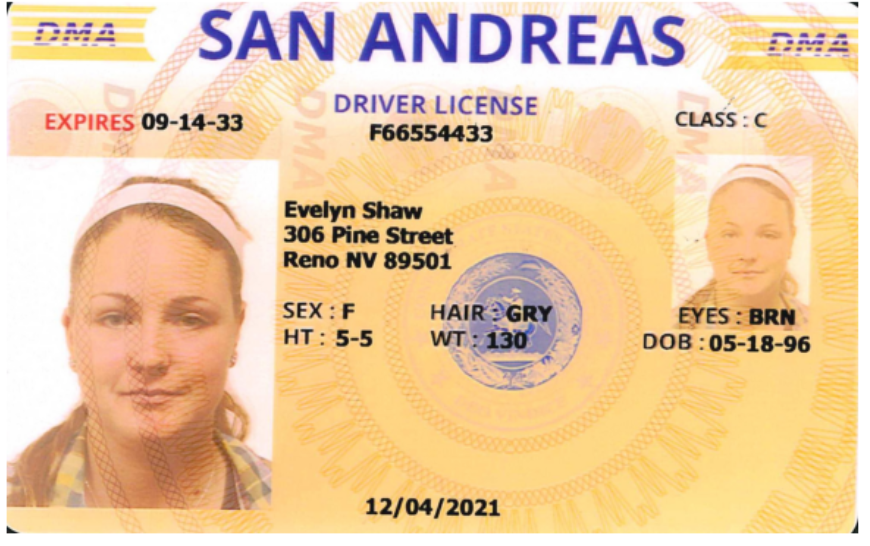
\includegraphics[width=0.318\textwidth]{figures/fig_qual_bonafide_input} &
    
\includegraphics[width=0.318\textwidth]{figures/fig_qual_bonafide_mask}  &
    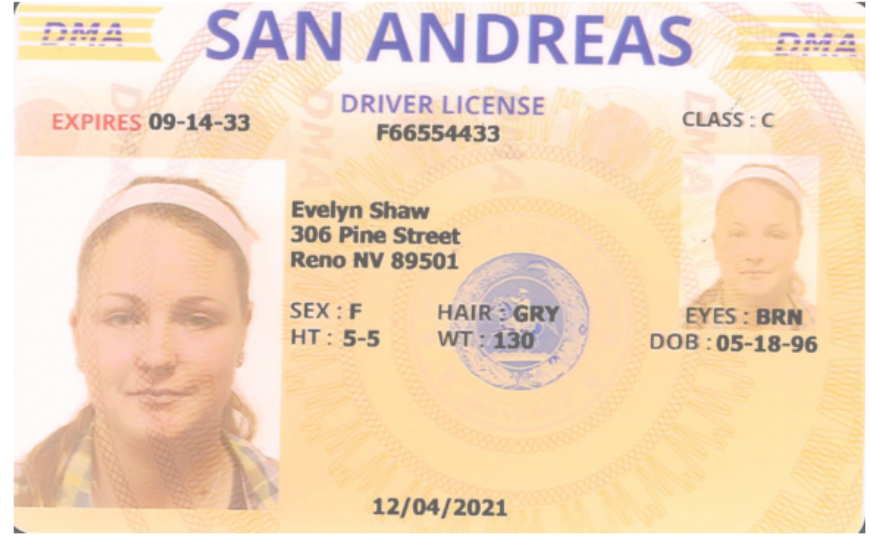
\includegraphics[width=0.318\textwidth]{figures/fig_qual_bonafide_overlay} \\[1pt]
    \multicolumn{3}{c}{\small (a) Bonafide document --- no alterations detected} \\[6pt]
    % --- Attack row ---
    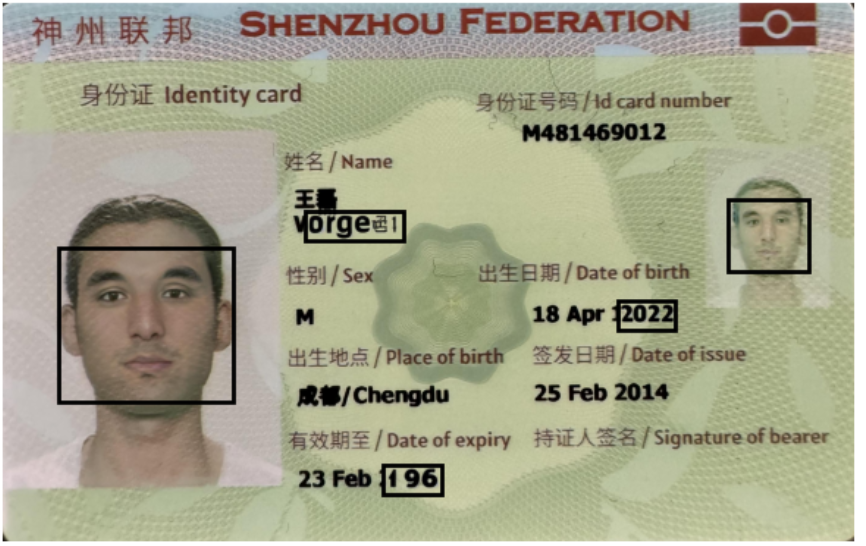
\includegraphics[width=0.318\textwidth]{figures/fig_qual_attack_input} &
    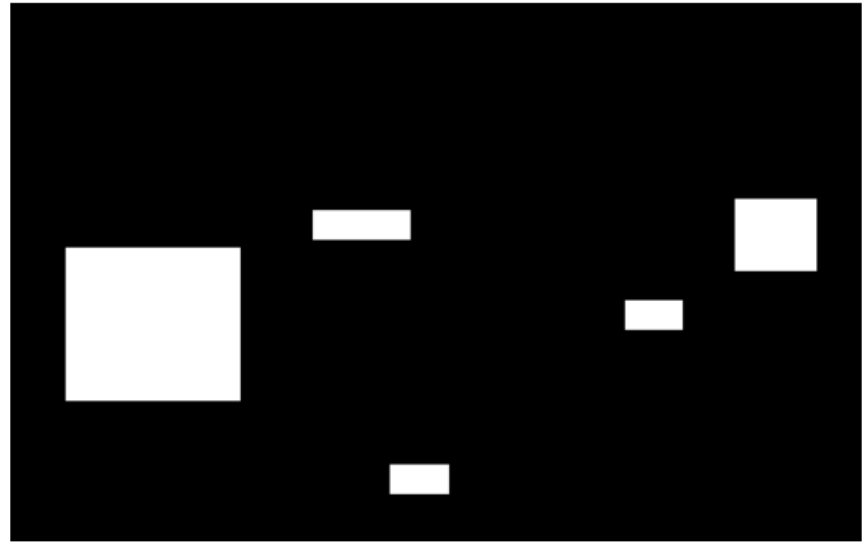
\includegraphics[width=0.318\textwidth]{figures/fig_qual_attack_mask}   &
    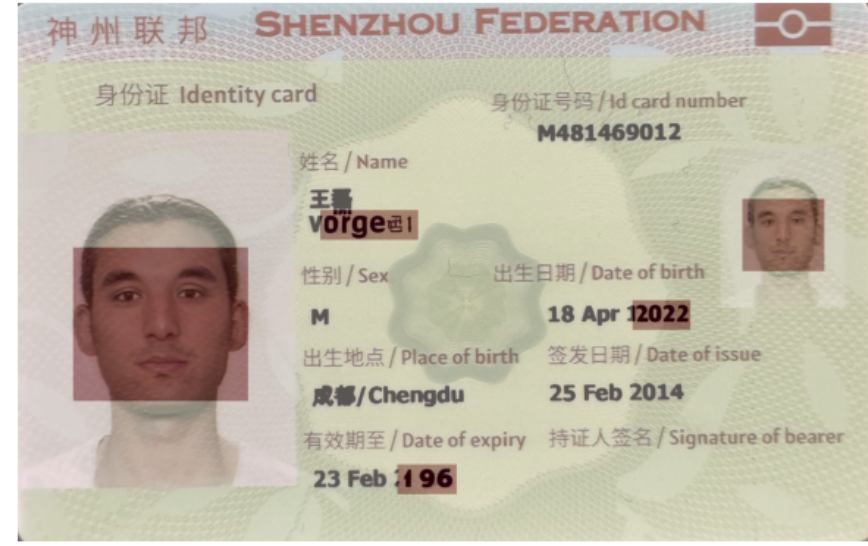
\includegraphics[width=0.318\textwidth]{figures/fig_qual_attack_overlay} \\[1pt]
    \multicolumn{3}{c}{\small (b) Forged document --- five altered regions localised} \\
  \end{tabular}
  \caption{Qualitative results on two FantasyID samples. \textbf{Left:} input
  document (forged regions framed in the attack sample). \textbf{Centre:} binary
  mask predicted by DocVerify. \textbf{Right:} input document with predicted mask
  overlaid in red.}
  \label{fig:qualitative}
\end{figure*}
